%(BEGIN_QUESTION)
% Copyright 2006, Tony R. Kuphaldt, released under the Creative Commons Attribution License (v 1.0)
% This means you may do almost anything with this work of mine, so long as you give me proper credit

Forklar hvorfor denne {\it 4-leder} RTD-kretsen er helt immun mot kalibreringsdrift som skyldes kabelresistans:

$$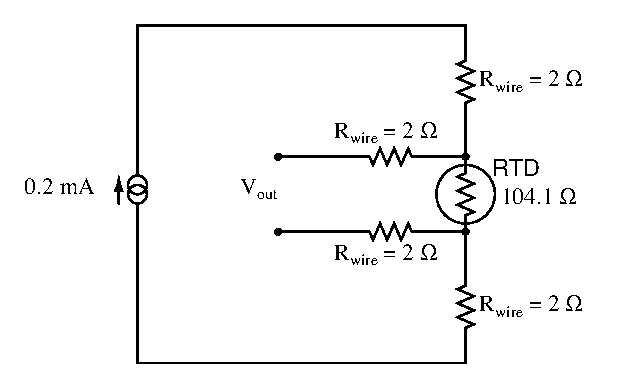
\includegraphics[width=15.5cm]{i00415x01.eps}$$

Identifiser også størrelse og polaritet for alle spenningsfall i denne kretsen.

\vskip 20pt \vbox{\hrule \hbox{\strut \vrule{} {\bf Forslag til sokratisk diskusjon} \vrule} \hrule}

\begin{itemize}
\item{} Hvordan vil temperaturmålingen påvirkes hvis strømkildens verdi økes?
\item{} Vil denne kretsen være immun mot kalibreringsdrift selv om RTD-ledningsresistansene ikke er like? Gjelder dette også for en 3-leder RTD-krets?
\item{} Forklar betydningen av DC-kildesymbolet brukt i diagrammet. Hvilken type kilde er dette, og hva er polariteten?
\item{} Velg en vilkårlig motstand i kretsen og tenk at den feiler (enten avbrudd eller kortslutning). Vil denne elektriske feilen få RTD-en til å se varmere ut enn den faktisk er, eller kaldere? Forklar svaret i detalj.
\end{itemize}

% CHANGE THIS TO A FAULT ANALYSIS QUESTION???

\underbar{file i00415}
%(END_QUESTION)





%(BEGIN_ANSWER)

%(END_ANSWER)





%(BEGIN_NOTES)

$$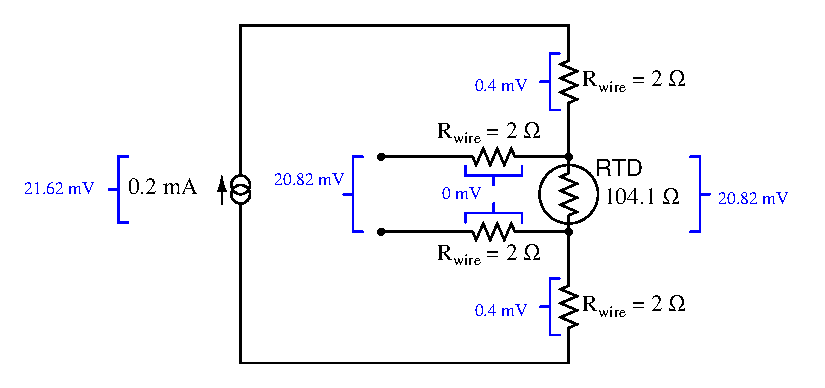
\includegraphics[width=15.5cm]{i00415x02.eps}$$

\vfil \eject

$$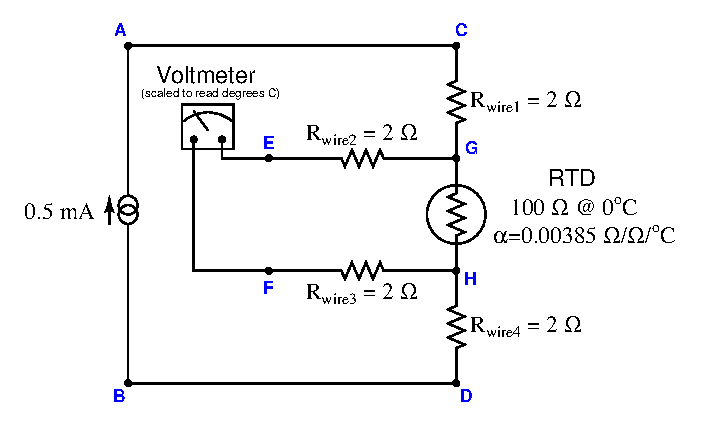
\includegraphics[width=15.5cm]{i00415x03.eps}$$

\vskip 20pt \vbox{\hrule \hbox{\strut \vrule{} {\bf Virtuell feilsøking} \vrule} \hrule}

Dette spørsmålet egner seg godt som en «virtuell feilsøking»-øvelse. Når du presenterer kretsdiagrammet for studentene, ser du først for deg en bestemt feil i systemet. Deretter presenterer du ett eller flere symptomer på denne feilen (noe en operatør eller annen bruker kan observere). Studentene foreslår så ulike diagnostiske tester for å identifisere feiltype og feilsted, som om de var teknikere som feilsøkte systemet. Din oppgave er å fortelle hva resultatet ville blitt for hver foreslåtte test, og dokumentere resultatene slik at alle studentene kan se dem.

Under og etter øvelsen er det nyttig å stille oppfølgingsspørsmål som:

\begin{itemize}
\item{} Hva forteller resultatet av den siste diagnostiske testen om feilen?
\item{} Anta at resultatet av den siste testen hadde vært annerledes. Hva ville det i så fall fortalt om feilen?
\item{} Er den siste diagnostiske testen den beste vi kunne gjort?
\item{} Hva ville vært den ideelle testrekkefølgen for å finne feilen i færrest mulig trinn?
\end{itemize}

%INDEX% Measurement, temperature: RTD (4-wire with cable resistance)

%(END_NOTES)
